% !TEX TS-program = pdflatex
% !TEX encoding = UTF-8 Unicode

% This is a simple template for a LaTeX document using the "article" class.
% See "book", "report", "letter" for other types of document.

\title{Understanding fetching performance on a core-fusion enabled processor}

\section{Setup}
In this section we will use a 16 core EDGE CPU and vary the number of segment lanes it can have.
Lanes define the number of blocks that can be in flight in parallel on a single core.
As an EDGE block can be a maximum of 128 instructions, each lane in a core will only be able to fetch a block which is 128/number of lanes large.
In the rest of the report I will use $E\textit{i}_n$ where i is the number of fused cores and n is the number of segments.

Throughout the rest of the report we assume a perfect L1 cache, so a block can be fetched in 1 or 2 cycles.

In this report we will see how having more lanes is, at least for a single core, advantageous due to the average size of a block.
However, as we will discover, this increases the overhead when it comes to core fusion, at least in its current form.

\section{Fetching overhead}
\subsection{On a single core}

The fetching procedure in a single core, $E1_4$ the fetching procedure behaves like this:

In a $E1_4$, as long as the core has a block in flight, it will attempt to fetch a new block every cycle.
A new block can be fetched as long as the header of the previous block has been decoded, which helps mask the latency of fetching a block from Icache.
With this information in hand, the fetch steps can be described as following:
\begin{itemize}
\item Cycle 1: Fetch block header
\item Cycle 2: Decode block header
\item Cycle 3: Make branch prediction
\item Cycle 4: Fetch new header.
\end{itemize}
A single core therefore requires, at minimum, about 10 cycles to fetch 4 block headers.

\subsection{On a core-composition}

When fusing cores, the current model used is defined as followed: Core $C_n$ will fetch blocks until it has filled all its segments; once this has been satisfied, it sends a prediction to $C_{n+1}$.
If $C_{n+1}$ currently has no blocks it will simply wait until it is sent a prediction.

To illustrate how this can become a problem I have profiled the twolf\_1 microbenchmark described here bellow:
\begin{lstlisting}
for (i = 0; i < loopcount; i ++)
{
    delta_cost = 10 - i * 100 /loopcount;
    fred =  ((double) delta_cost * cost_scale_factor ) / T ; 
    if( fred >= 0.0 ) 
        truth = 1 ;
    else if( fred < -80.0 )  
        truth = 0 ;
    else if( fred > -0.0001 ) 
    {
        if( 1.0 + fred > ( (double) RAND / (double)0x7fffffff ) )  
            truth = 1 ;
        else 
	 truth = 0 ;
    }
   else 
   {
         fract = (int)( -fred * 8388608.0 ) ;

          if((table1[ (fract >> 20) & MASK ] * 
              table2[ (fract >> 10) & MASK] * 
              table3[ fract & MASK ]) > 
              ( (double) RAND / (double)0x7fffffff ) ) 

                  truth = 1 ;
         else 
            truth = 0 ;
    }
}
\end{lstlisting}

The reason I chose this benchmark is due to the small blocks it will generate.

\begin{figure}
\center
  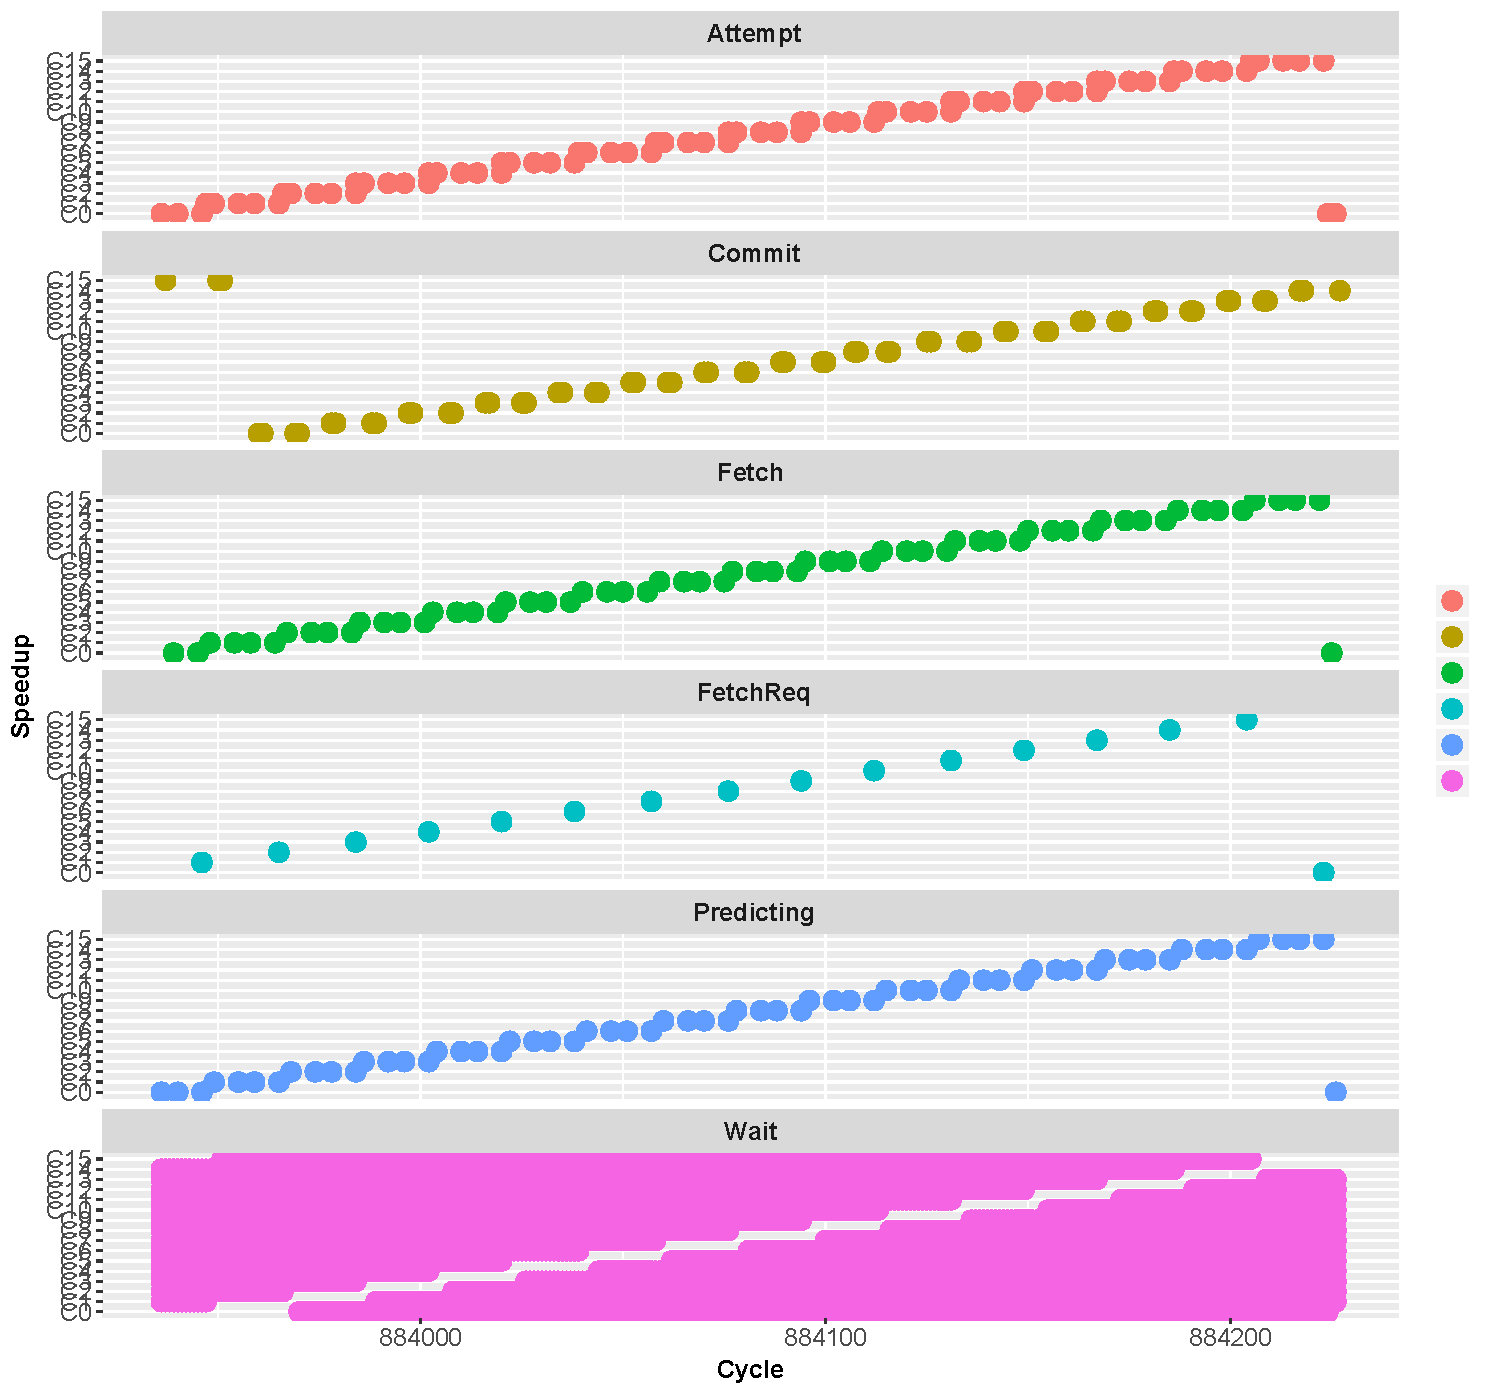
\includegraphics[width=1\textwidth]{chapter3/graphics/twolf_16.pdf}
  \caption{TWOLF on 16 cores fused, 4 segments each}\label{fig:16step}
\end{figure}

\begin{figure}
\center
  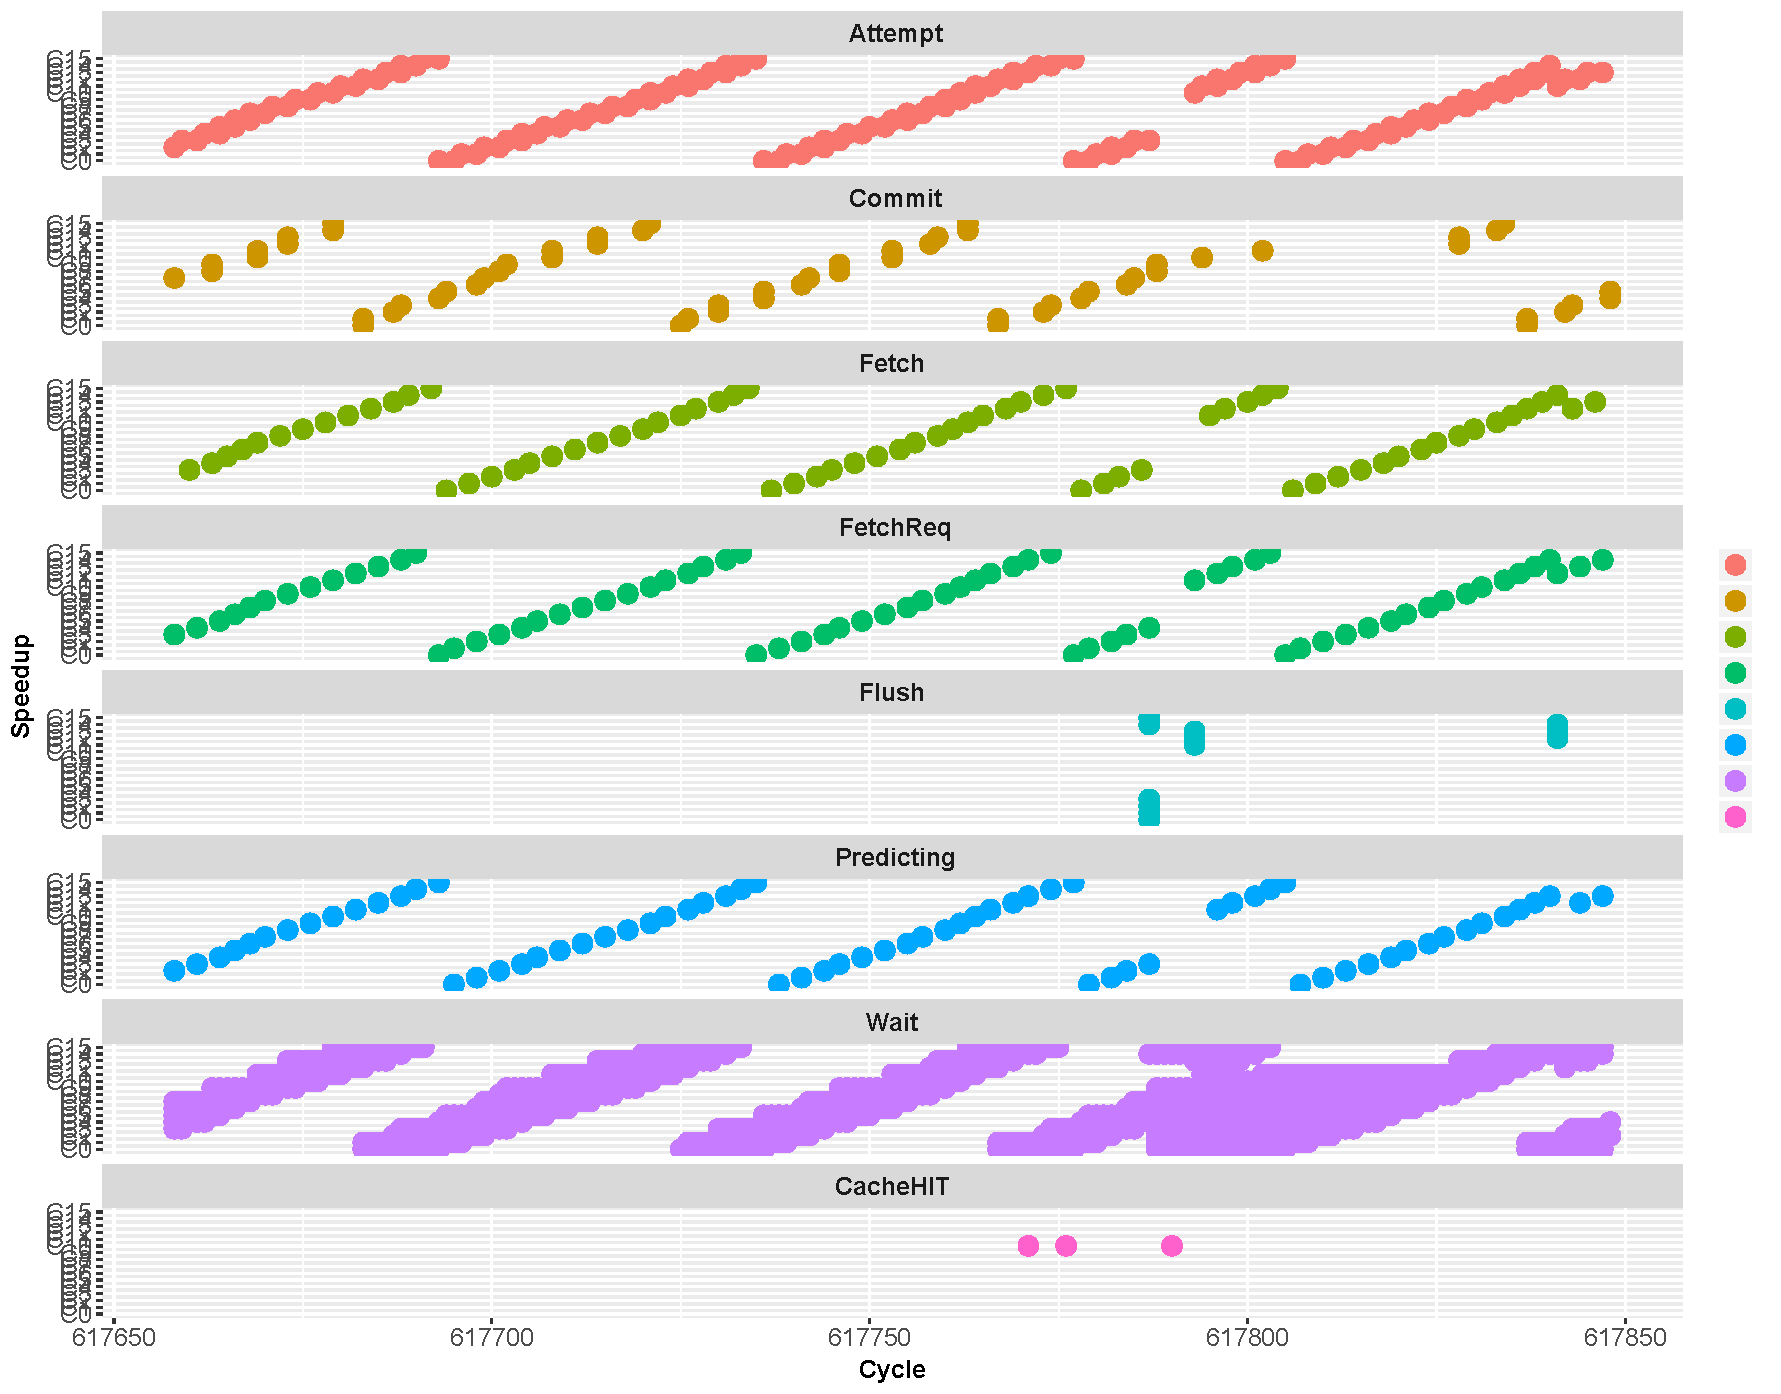
\includegraphics[width=1\textwidth]{chapter3/graphics/twolf_16_1.pdf}
  \caption{TWOLF on 16 cores fused, 1 segments each}\label{fig:16step1}
\end{figure}

\begin{figure}
\center
  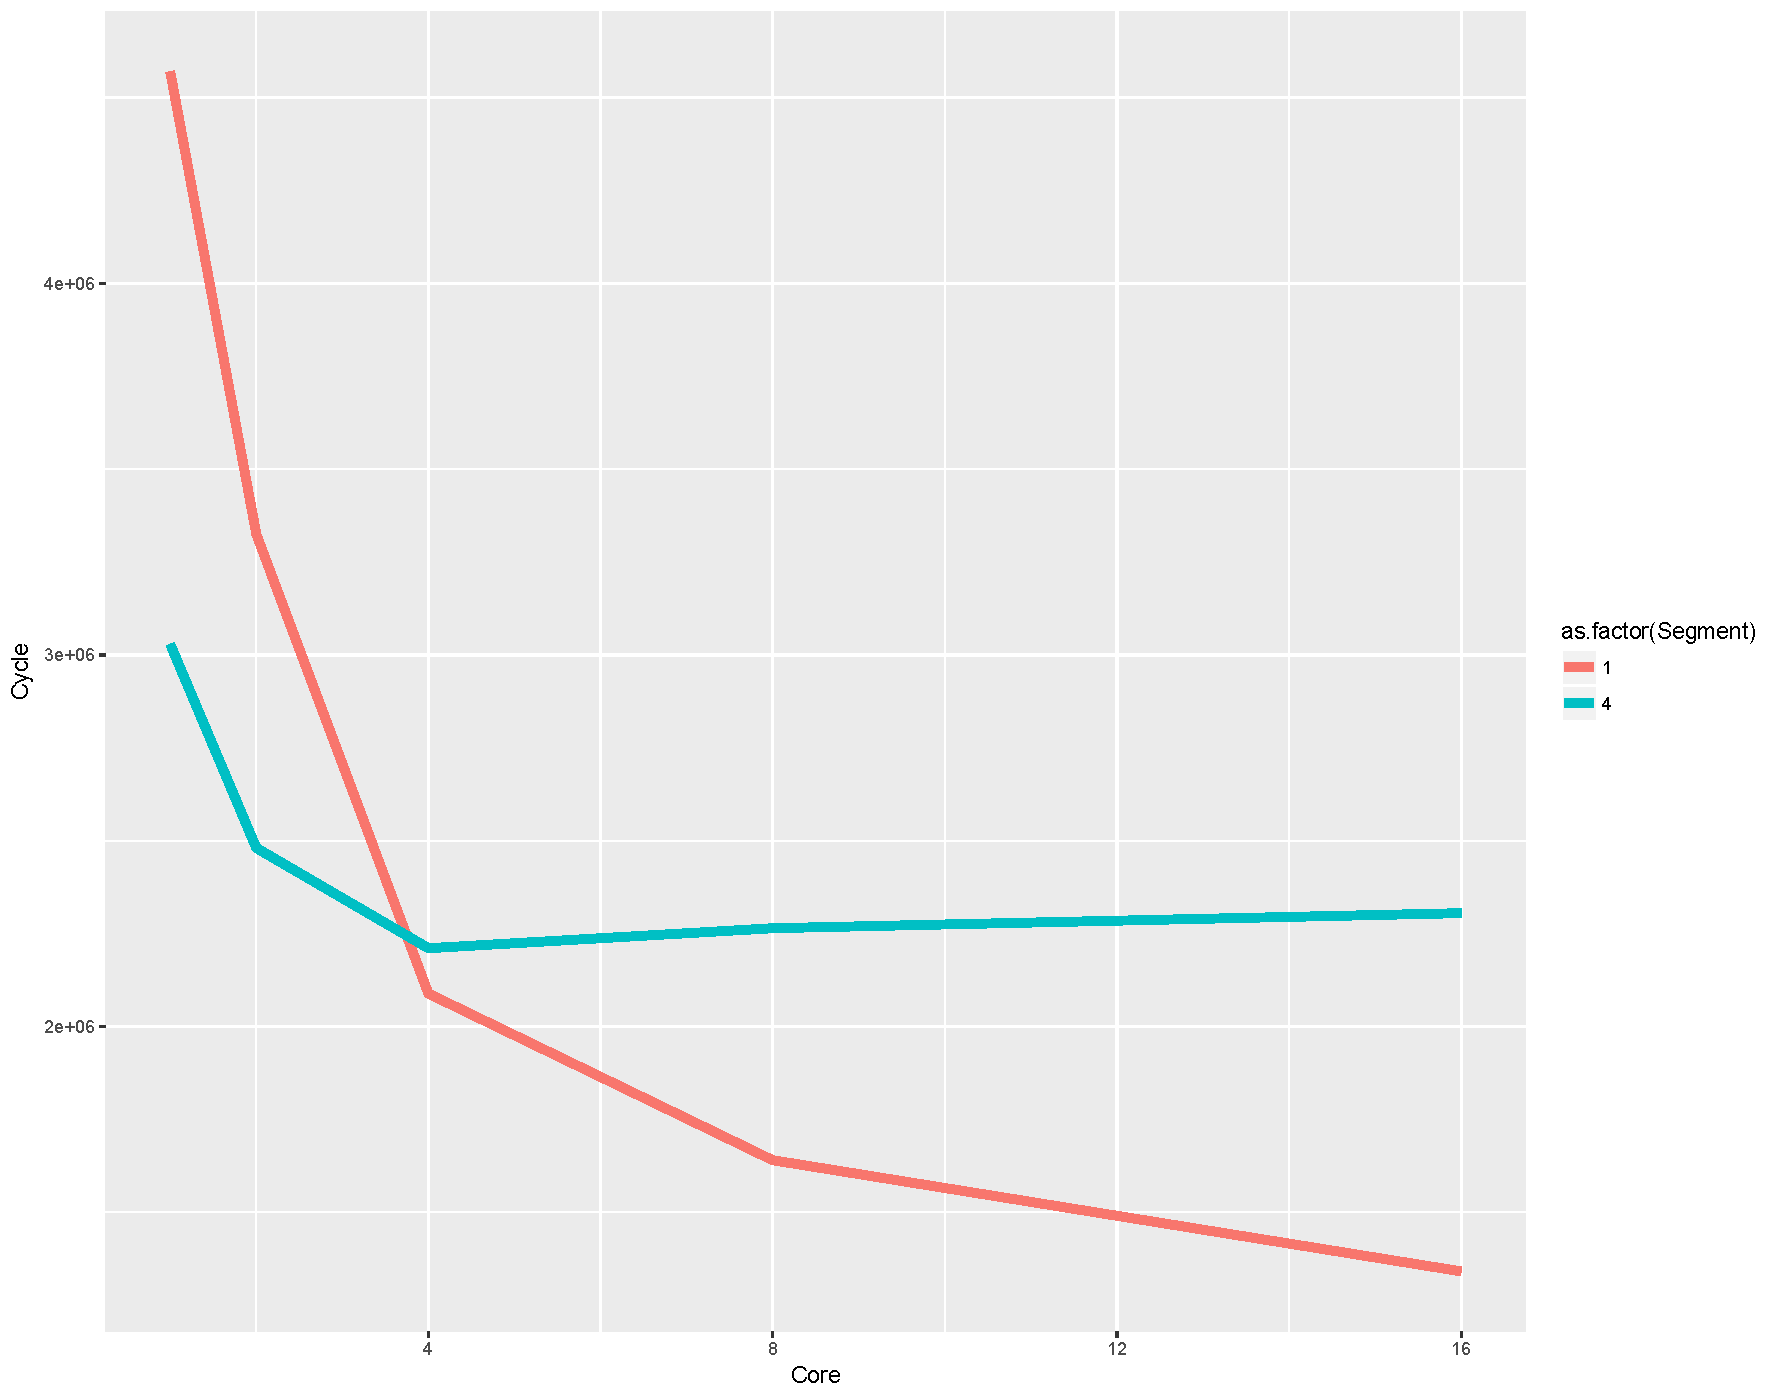
\includegraphics[width=1\textwidth]{chapter3/graphics/twolf_perf.pdf}
  \caption{Cycle comparison for 1 or 4 segments}\label{fig:4v1}
\end{figure}
Figure~\ref{fig:16step} represents the execution of 64 blocks for 16 cores fused, the Y axis represents each core, and the X axis is the cycle.
Each of the facets of the graph are defined here:
\begin{itemize}
\item Attempt: Block is attempting to allocate a new block
\item Commit:  Cycle where a block is being commited
\item Fetch: Cycle where a new block is being fetched
\item FetchReq: Cycle where a core is receiving a fetch request from another block.
\item Predicting: Cycle where a core makes a block prediction.
\item Wait: Cycle where core is in execution stage but there are no blocks in its segments.
\end{itemize}

We can clearly see how inefficient this is simply by looking at how, for almost 90% of the execution of the 64 cores, each core is simply waiting.
In fact, when looking at when cores are not waiting around, we can clearly see almost no overlap of execution between cores, meaning that the cores are never actually executing in parallel.
Since the blocks are not long enough, the overhead of fetching and dispatching blocks to multiple cores is clearly overtaking the usefulness of having this many cores.

In Figure~\ref{fig:16step1} we have an $E16_1$ running a similar section of TWOLF (getting the extact section is hard due to the difference in branching), and we can see that, when executing a single segment, the cores will have more execution time being interleaved. This is to be expected as the overhead of fetching and dispatching a single block for each core is less than 4 blocks per core.
In fact, Figure~\ref{fig:4v1} we can see that having only a single segment will outperform 4 segment cores after 4 fused cores.
The reason is once again due to how blocks are scheduled: in a single segment core, we know that each block will be executed in parallel, and each core will have a block fairly quickly.
Naturally, on a smaller cluster having 4 segments can be more advantageous as the fetch latency wont be as high.

\newpage
\subsection{Comparing segment performance}

Bear with me on this one.
In this section I want to demonstrate how average cycle count of a block affects potential speedup based on the number of segments and number of cores fused.
Unlike in CASES paper where I simply wrote a small math equation to measure maximum IPC, here I ran a small microbenchmark which contained a single instruction.
In this scenario, I could run a simulation where I could define the execution time of that instruction in cycles.
Using this, I ran a set of experiments where I modified the number of segments, 1 or 4, number of cores fused (1,2,4,8,16) and the length of the block (10,20,40,80,160,320).
I've generated 2 figures here, Figure~\ref{fig:lss} represents the speedup relative to segments.
In other words I grouped executions with the same segments to calculate the speedup.
As we can see, for a core fusion of 16 cores with 1 segment to get a 16x speedup compared to 1 core with 1 segment, we would need independent blocks of at least 40 cycles in length.
By logging fetch requests for each core, I've noticed it takes 39 cycles for 16 cores to have their blocks (in this example).
Since each block takes 40 cycles, this means that by the time Core 1 will have finished executing its block, Core 15 will have fetched and submitted a prediction.
This is an ideal situation as cores are therefore always executing blocks, leading to a full utilisation.

On 4 segment cores, the picture is much less appealing; it takes blocks of length 160 to get a 14x speedup.
By doing the same kind of logging as I did before, I see that with four segments, we take about 180 cycles to fill up all cores, so that means each block would at least have to be 180 cycles to be useful. 
Whilst this may come to no surprise, it shows that we need blocks to be at least 4x longer on a 4 segment machine compared to single segment.

So what's the point of 4 segment cores then ? It's easier to demonstrate the usefulness of core-fusion on single segment CPUs.
This may be correct, but as we can see in Figure~\ref{fig:ts} where I compare the cycle counts of all executions to 1 Core 1 Segment; having 4 segments can be very beneficial.
Indeed, on longer blocks, (160 and beyond) we could, in theory, be getting up to a 64x speedup with 16 cores and a 4x speedup with just one core!
Naturally this is purely theoretical, but there coudl be cases where this happens.
Having more segments not only should allow us to accomodate for smaller blocks, but also enables us to ensure that the cores can issue instructions at a more steady rate, as they can look for any available instruction from 4 blocks instead of a single 1.
Ironically this also shows that larger isn't always better, if we could generate 4 blocks that are perfectly independent and populate 16 cores with those blocks, we would technically get a better speedup than if we had 1 large block!

\subsubsection{Small caveat}

In this example, the block is only 1 instruction large, which makes the fetching extremeley quick.
Even though I use a perfect ICache, we have a single cycle here to fetch all the instructions needed.
I think that if the blocks are larger this will affect fetching performances (making them slower) and increasing the required length of a block.

\begin{figure}
\center
  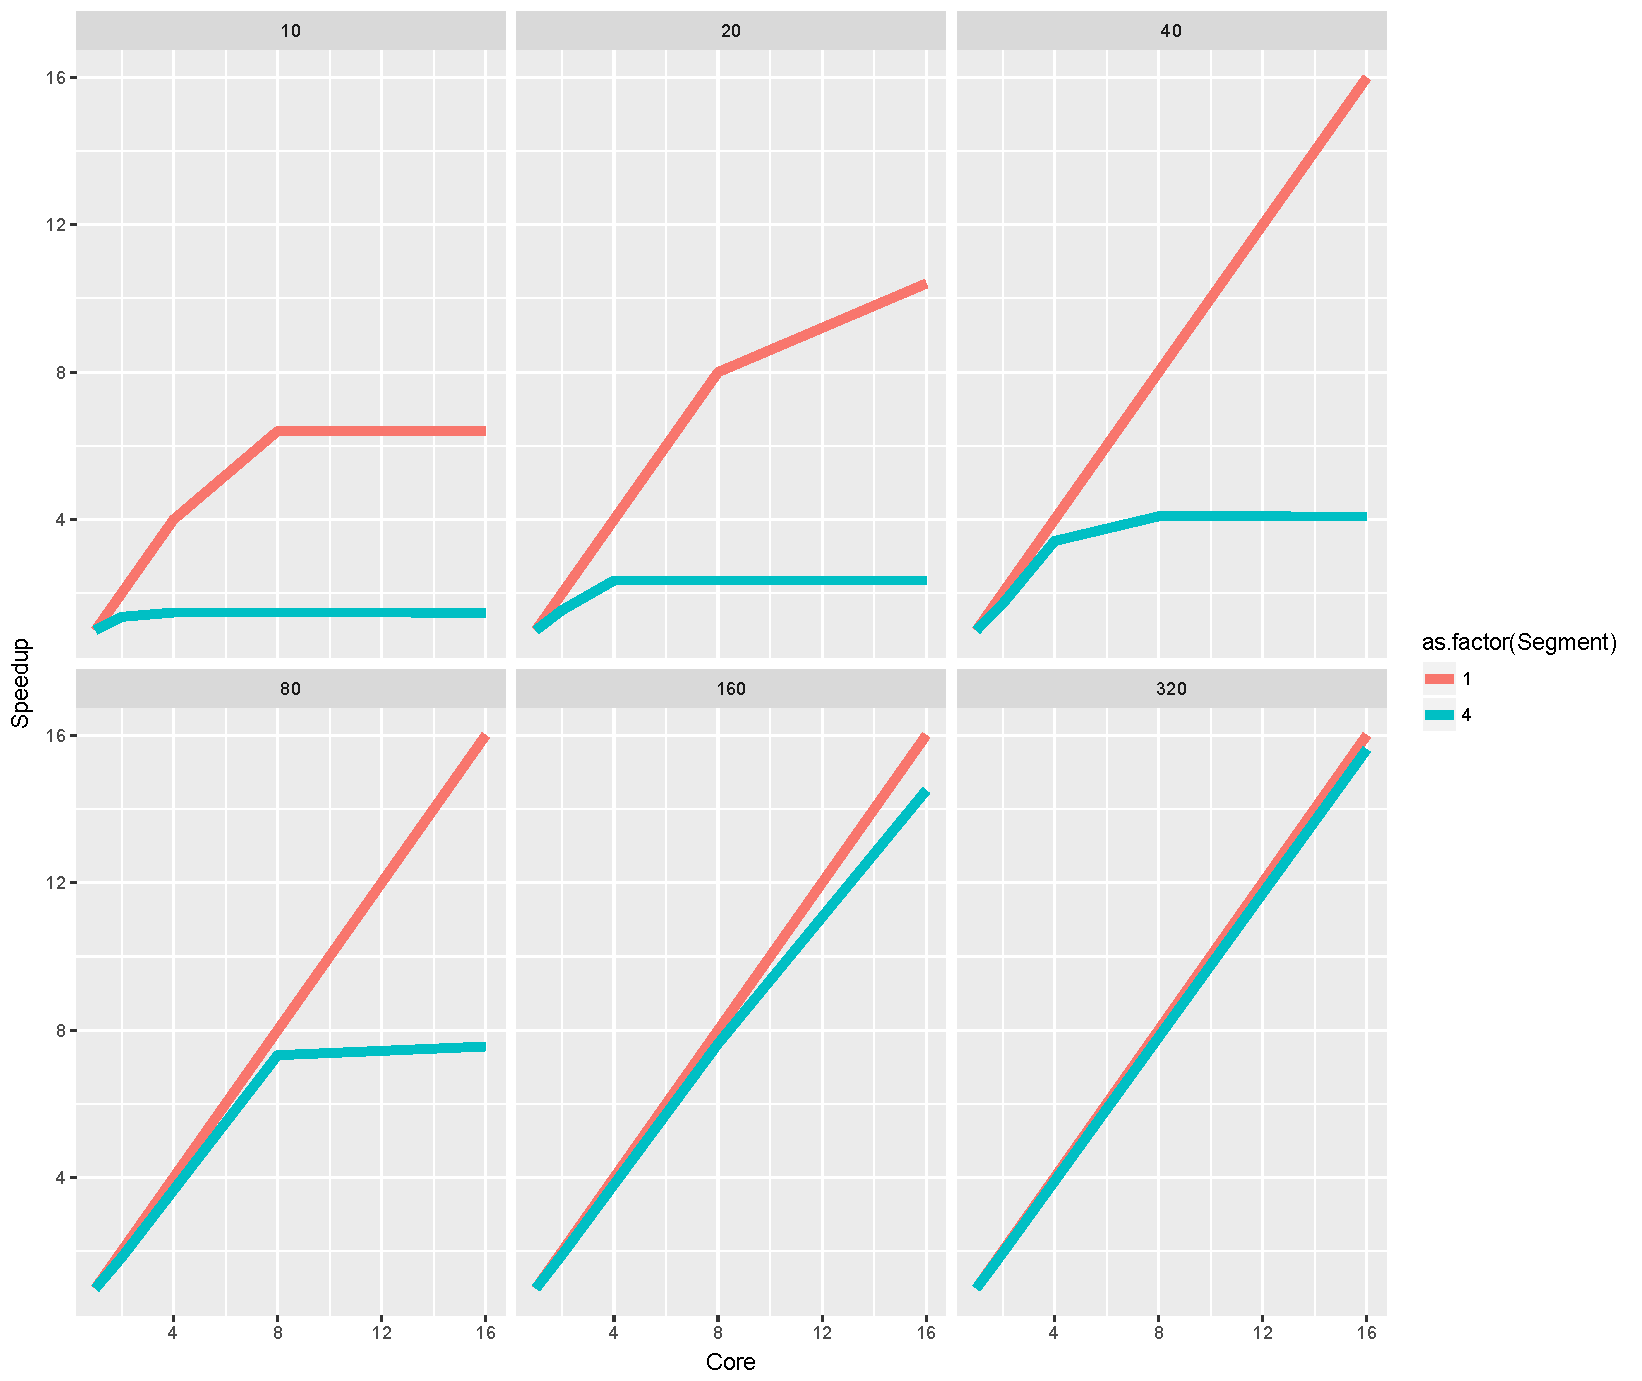
\includegraphics[width=1\textwidth]{chapter3/graphics/lengths_segment_speed.pdf}
  \caption{Speedup by segments.}\label{fig:lss}
\end{figure}

\begin{figure}
\center
  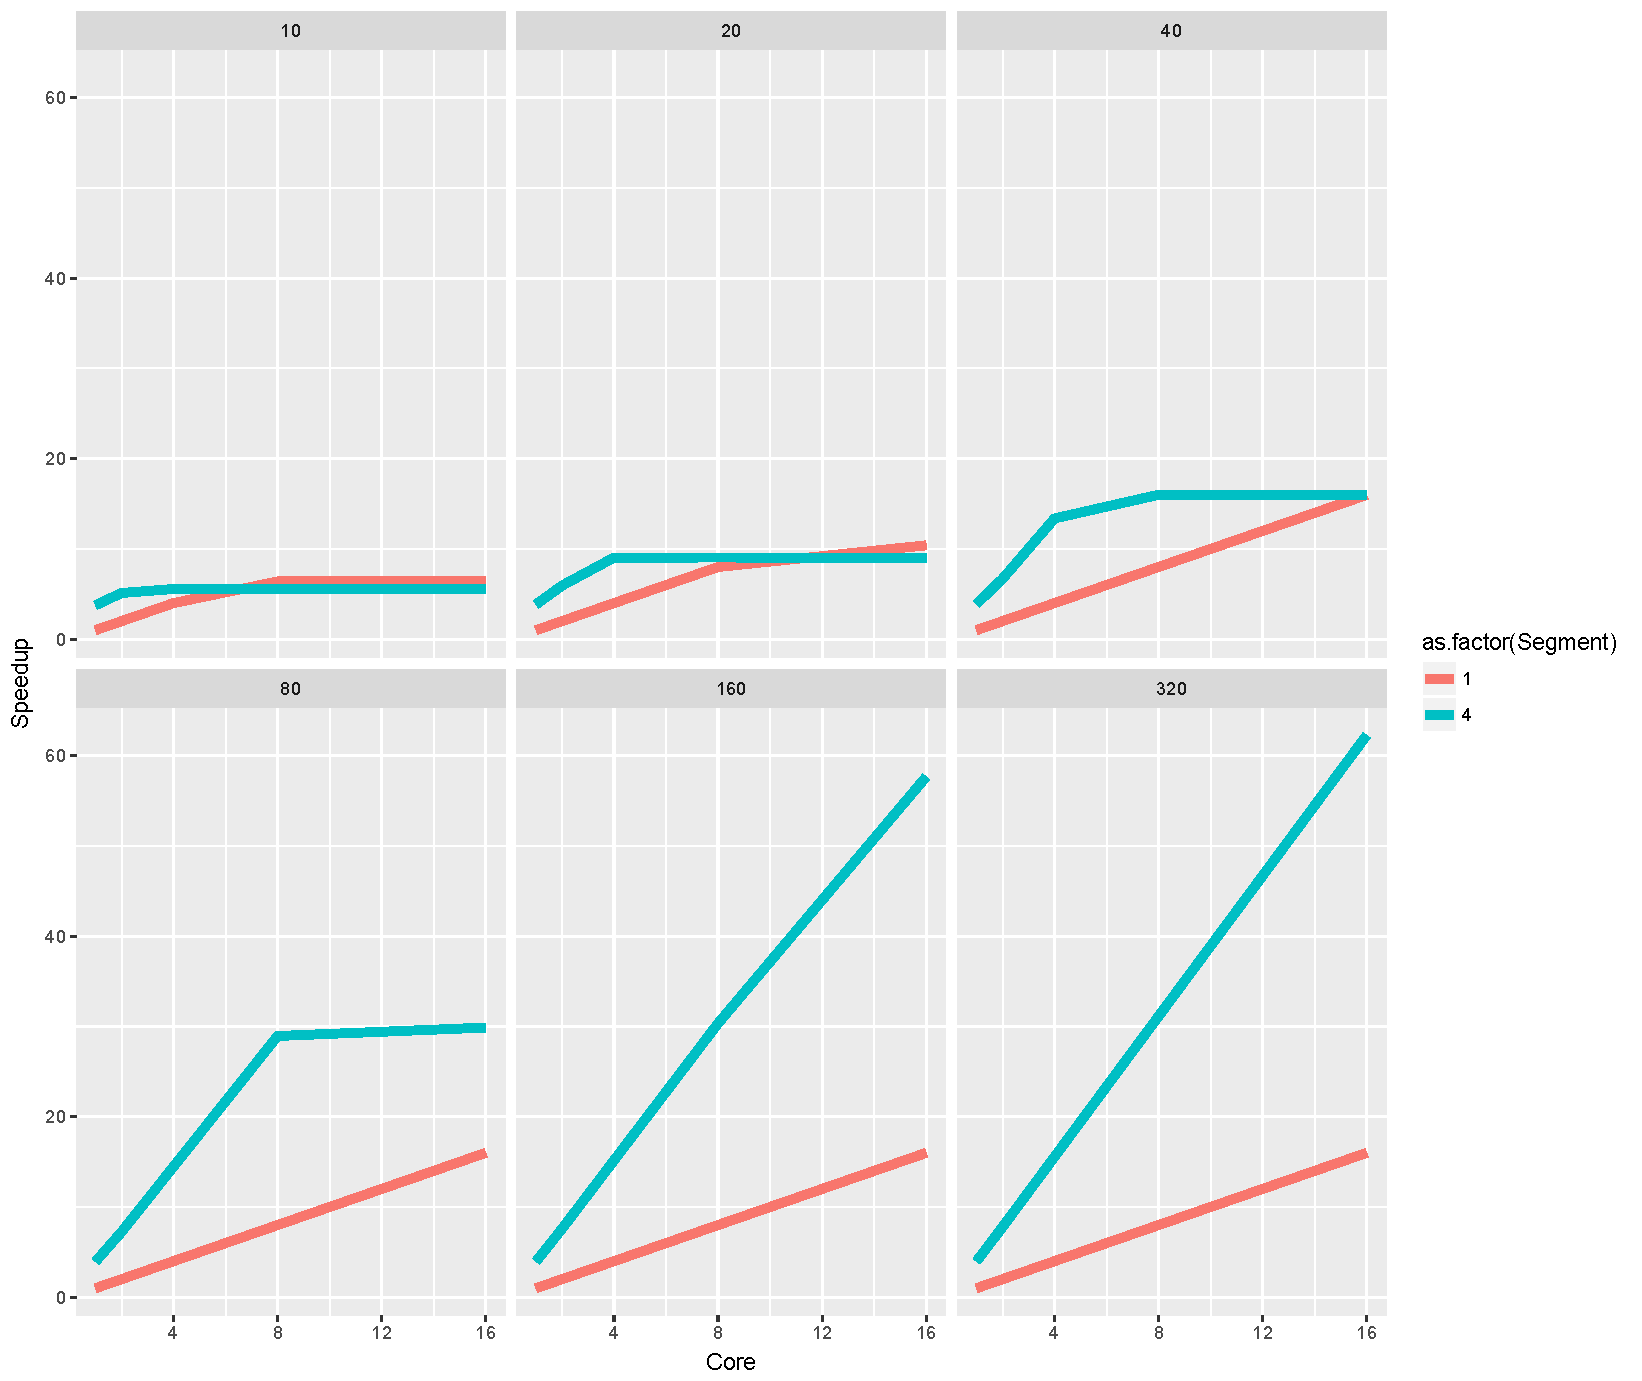
\includegraphics[width=1\textwidth]{chapter3/graphics/total_speed.pdf}
  \caption{Maximum speedup compared to 1 Core 1 Segment}\label{fig:ts}
\end{figure}


\section{How core-fusion models do it}
\subsection{EDGE}
We just described it, but again here it is:
As it exists now, each core in a composition will fetch blocks until they're full, and then submit the subsequent block to another core.
When a core no longer has the youngest segment it will wait for a core in the composition to send it a block.

\subsection{Core-Fusion, Ipek et. al}

Core-Fusion has a Fetch Management Unit (FMU) that allows it to dispatch instructions to cores in a composition.
An FMU will receive information from a core and resends relevent fetch information to other cores in the composition.
Usually the latency from 1 core to another via the FMU is 2 cycles.

In Core-Fusion, the cores independently fetch instructions from their Icache. They can fetch, at best, 2 instructions per cycle and have a max capacitiy of 8 instructions.
The cores in a fusion will be dependent on Core-Zero for fetch alignment.
When a fetch-stall occurs, such as an i-cache miss or i-tlb miss, all cores must stall to ensure correct alignment.
Each core can conduct a single prediction per cycle, it will send those predictions/mispredictions to the FMU which selects the correct PC to inform all cores about where to fetch.
A mispeculation will cause flushing of all cores, naturally.

In their situation, the overhead of fetching is supposedly negligeable, for example on an 8 Core system it's only 3\% on SPECINT/SPECFP.
However most of their time is spent in pipeline stalls, which most likely isn't alieviated by the fact that, at best, each core can only have 8 instructions running at any point.

\subsection{Baharupi, Pricopi et. al}
This is similar to EDGE but it doesn't use the block structure.
Instead, there's a "Sentinel Instruction" which acts like a block header, informing the core on whether or not the basic block ends with a branch/fallthrough.
When a core fetches a sentinel instruction it will execute a branch and submit it to the next core in the composition.
So this is similar to EDGE with single segment.
It's slightly less efficient due to the fact that the cores do live register renaming and depend on a shared General Program Counter (GPC).
Cores can't submit blocks in parallel, instead they need to lock in the GPC when they hit a sentinel instruction.
The GPC will be locked until register renaming is finished and the branch prediction is done.
This adds an extra latency as cores will simply have to wait for these procedures to be done to get ahold of the GPC.

\subsection{Conclusion}
Most core-fusion models operate in a similar manner, that is to say cores communicate with each other via some form of branch prediction / fetch manager to determine which instructions to fetch.
Baharupi introduces a lock on a General Program Counter which can cause extra latency due to cores needing to get the lock.
Core-Fusion claims to have a very small overhead, but this is also due to the fact that each core is only ever fetching a maximum of 2 instructions per cycle.
Given that they worked with an 8 core system that means they have a maximum of 64 instructions in flight at any point.
Since cores don't require a new branch prediction to fetch instructions, this can considerably reduce the overhead of the fetching model.
This is nothing compared to what EDGE can potentially do; on an 8 Core fusion we could have 1024 instructions being fetched, which could be a result of 8 to 32 fetch requests.

Ultimately EDGE requires branch predictions like Baharupi but doesn't suffer from lock-acquiring stalls.
However, unlike Core-Fusion, we cannot simply fetch instructions in parallel as we require to have decoded headers and made predictions as to what the next block will be, which increases the latency when we have more segments and cores.

\section{What can we do about it?}

\subsection{Unlocking block dispatch}

Currently a core cannot issue a new block if its youngest segment has already submitted a fetch request.
This current restriction means that blocks have to be submitted to cores in a sequential fashion, in other words, if we have 2 cores in a fusion, then C1 cannot fetch a block, send another block to C2 and then fetch a 3rd block. Instead, once it has submitted a block to C2 it will \textbf{have} to wait for C2 to send a new block.
This is what is currently causing cores to wait. Once they have submitted a block to another core, even if their youngest segment commits, they must wait for all other cores in the composition to have fetched blocks so that the fetching wraps back to it.

What I propose as a first step is to try and explore new fetching mechanisms for core-fusion, mainly pipelining fetches.
Instead of "fetching until you're full", a core should start off by making 1 prediction for itself and 1 prediction for the next core in the fusion.
Once it has executed this step it can continue fetching 3 other blocks whilst the next core repeats the process.
This should ensure all cores are fetching 4 blocks almost in parallel.
A paper from 1996 by Andre Seznec et al. from INRIA proposed a multi-block branch predictor that can generate 2 predictions in a single cycle.
We could use this work to do predictions for number of blocks.

Currently, if we have 16 cores, each fetching 4 blocks, if we assume that it takes at least 4 cycles to fetch a block and send a prediction, we have
$fetchlat=(16 * 4)*4$  so 256 cycles before each core has filled up.
By pipelining we can reduce this down to $fetchlat=4+(15*4)+4$  so 68 cycles which is a 3.7x speedup.
Refering back to Figure~\ref{fig:lss}, having an overhed of 68 cycles would place us between the 40 and 80 cycles facet, which means that if we are able to maximize speedup around those facets, that's a 2.6x speedup for a 16 core, 4 segment fusion.
This should, in theory, allow us to better utilise core-fusion as it decreases the restrictions on how long a block should take to execute for a given core-composition size.
Let's recall in the previous report that the overall speedup of a loop, when we only have a single segment can be measured by:
\begin{equation}\label{eq:avspeed}
\frac{Average Execution Time}{\frac{4+4*(Cores -1)+ Average Execution Time + Dependencies  * Cores}{ Cores}}
\end{equation}

In this formula, $4+4*(Cores-1)$ represents the fetch overhead when we have a single segment.
Currently, on 4 segments this would be $4+4*(Cores-1)*4$ which reduces the potential speedup window.

\subsection{Improving branch prediction requirements}

We can use this oportunity of exploring how blocks are fetched to improve overall core-utilisation by ordering the blocks in a different manner.
As we state in the CASES paper, for a core to be useful in a core-fusion, all previous blocks must have been accurately predicted, which can be a huge strain on the branch predictor.
If, instead, we were to send the first prediction made by a core to the following core, we can reduce the stress on the branch predictor.
For example if we had 4 Cores, C1 would have blocks [1,5,9,13] C2:[2,6,10,14], C3:[3,7,11,15] and C4:[4,8,12,16].
In this case, we only need to make 3 predictions to ensure that C4 has at least been somewhat useful.
Previously, in a 16 core composition, if we had 64 blocks in flight, the 16th core could only be considered useful if 60 out of the 64 blocks were considered correct.
This implied at least a 93.7\% accuracy just to ensure that all cores were running some correct code whereas in this new model, only 15 predictions would ensure a utilisation of the core, so dropping it to a mere 23\%.
In Core-Fusion by Ipek et al. Figure 9 shows the distribution of fetch cycles for SPECINT and SPECFP benchmarks.
They define 4 categories: pipeline stalls (cores are busy executing), wrong path (misprediction), FMU stalls (stalls caused by communicating to FMU) and true fetch, which I assume is cycles spent doing actual fetch work.
Whilst they claim that the FMU only causes a 3\% overhead in fetch cycles, they fail to address the fact that, for some benchmarks in SPECINT, mispeculation can caust them up to 50\% of their fetch cycles which is huge.
In these cases they percieve no speedup since they're getting branches wrong almost half the time.
By changing the scheme we can claim that we maintain a higher number of live blocks whilst allowing cores to be useful more frequently.

\subsection{Exploring smarter schedulers}

A lot of the talk in this report is somewhat focused on trying to tackle fetching overhead when we assume blocks are small and take no time to execute.
This most often will only occur in integer heavy blocks, or situations where all data is in cache and blocks are small due to heavy control flow.
However this isn't always the case, and blocks can take a long time to execute.
In these situations, the overhead of fetching isn't the problem but rather which blocks are being fetched and dispatched.
Since we're playing around with how blocks are dispatched we may use this oportunity to look at loops 
